\documentclass[aspectratio=169,11pt]{beamer}
\graphicspath{{figures/}} % Setting the graphicspath

% Theme settings
\usetheme{Madrid}
\usecolortheme{default}
\setbeamertemplate{navigation symbols}{}   % removes navigation symbols such as 'next page'
\setbeamertemplate{footline}{}             % remove line with name, date, page nr. 
\setbeamercolor*{frametitle}{bg=white}     % remove background from frametitle
\usepackage{caption}
% \captionsetup[figure]{labelformat=empty}% redefines the caption setup of the figures environment in the beamer class.
\setbeamersize{text margin left=20pt,text margin right=10pt}

\usefonttheme[onlymath]{serif} % makes beamer math look like article math


%======================= import packages =======================
\usepackage{pifont}       % Pi fonts (Digbats, symbol, etc.)
\usepackage{graphicx}     % More options for \includegraphics
\usepackage{appendixnumberbeamer} % separate appendix numbering
\usepackage{booktabs}
\usepackage{hyperref}
\usepackage{tabularx}
\usepackage{amsmath, nccmath}

%======================= define new commands =======================
\newcommand{\nn}{\vspace*{1em}}

%======================= page numbering =======================
\addtobeamertemplate{navigation symbols}{}{ \usebeamerfont{footline}
  \insertframenumber / \inserttotalframenumber \hspace*{2mm} \\ \vspace*{1mm} 
}


%=================================== colors ===================================
\definecolor{RoyBlue}{RGB}{22, 46, 69}
\definecolor{RoyGrey}{RGB}{64, 88, 128} 

\newcommand{\hlme}[1]{{\color{red}\bf #1}} % highlihgt me

\setbeamercolor{structure}{fg=RoyBlue} % itemize, enumerate, etc
\setbeamercolor{frametitle}{fg=RoyGrey}
\setbeamercolor{section in head/foot}{bg=RoyBlue}


%======================= add progress dots to headline =======================
\setbeamertemplate{headline}{%
    \begin{beamercolorbox}[ht=4mm,dp=4mm]{section in head/foot}
        \insertnavigation{\paperwidth}
    \end{beamercolorbox}%
}%
\makeatother


%======================= add section title page =======================
\AtBeginSection[]{
  \begin{frame}
  \vfill
  \centering
    \usebeamerfont{title}\insertsectionhead\par%
  \vfill
  \end{frame}
}


%=================================== titlepage ===================================
\title{Can the NNPDF model be simplified?}
\date{NNPDF Meeting, 6-8 September 2021, Gargnano}
\author{Roy Stegeman}
\institute{University of Milan and INFN Milan}
\titlegraphic{\vspace*{6mm}
  
\includegraphics[height=0.8cm]{logos/LOGO-ERC.jpg} \hspace{10mm}
	
\includegraphics[height=0.8cm]{logos/n3pdflogo_noback.png} \hspace{10mm}
	
\includegraphics[height=0.6cm]{logos/nnpdf_logo_official.pdf} \hspace{10mm}
	\includegraphics[height=0.8cm]{logos/Logo_Università_degli_Studi_di_Milano(not_mandatory).png}
	
\includegraphics[height=0.8cm]{logos/INFN_logo.png}
  \vspace*{5mm} \\
	\centering{ 
    \fontsize{7.0pt}{0.0pt}\selectfont This project has received funding from the European Union’s Horizon 2020 \\	
    \vspace*{-1mm}
    research and innovation programme under grant agreement No 740006.
	}
}


\begin{document}
{
\setbeamertemplate{headline}{} % remove headline from titlepage
\begin{frame}
  \titlepage
\end{frame}
}


%%%%%%%%%%%%%%%%%%%%%%%%%%%%%%%%%%%%%%%%%%%%%%%%%%%%%%%%%%%%%%%%%%%%%%%%%%%%%%%%%%%%%%%%%%%%%%%%%%%%
\section*{The NNPDF model}



\begin{frame}[t]{The NNPDF model}
  \only<1> {$$ xf_k(x) = A_k x^{1-\alpha_k}(1-x)^{\beta_k} \mathrm{NN}_k(x,\log x) $$}
  \only<2-> {{\bf Preprocessing} exists for historic reasons, it is still used to improve convergence and to model the extrapolation region. \\ \nn}
  \only<3-> {$(x,\log x)$ mixes objects with different orders of magnitude, which is poor practice from an ML standpoint \\ \nn}
  \only<2> {$$ xf_k(x) = A_k {\color{red} x^{1-\alpha_k}(1-x)^{\beta_k}} \mathrm{NN}_k(x,\log x) $$}
  \only<3-> {$$ xf_k(x) = A_k {\color{red} x^{1-\alpha_k}(1-x)^{\beta_k}} \mathrm{NN}_k({\color{red} x,\log x}) $$}
  \only<4> {\\ \vspace*{1.5cm} \bf \centering Can we simplify this architecture?}
\end{frame}


\begin{frame}[t]{A naive attempt}
  An obvious first attempt is $$ xf_k(x) = A_k \mathrm{NN}_k(x), $$ but this results in saturation of the activation functions:
  \begin{center}
    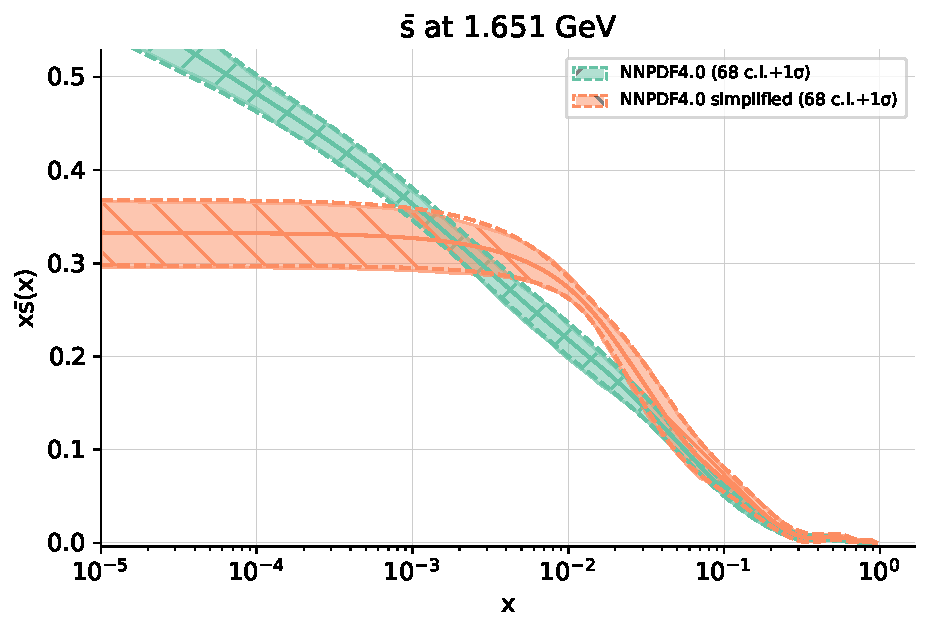
\includegraphics[height=0.55\textheight]{pdf_sbar_log_saturated.pdf} 
    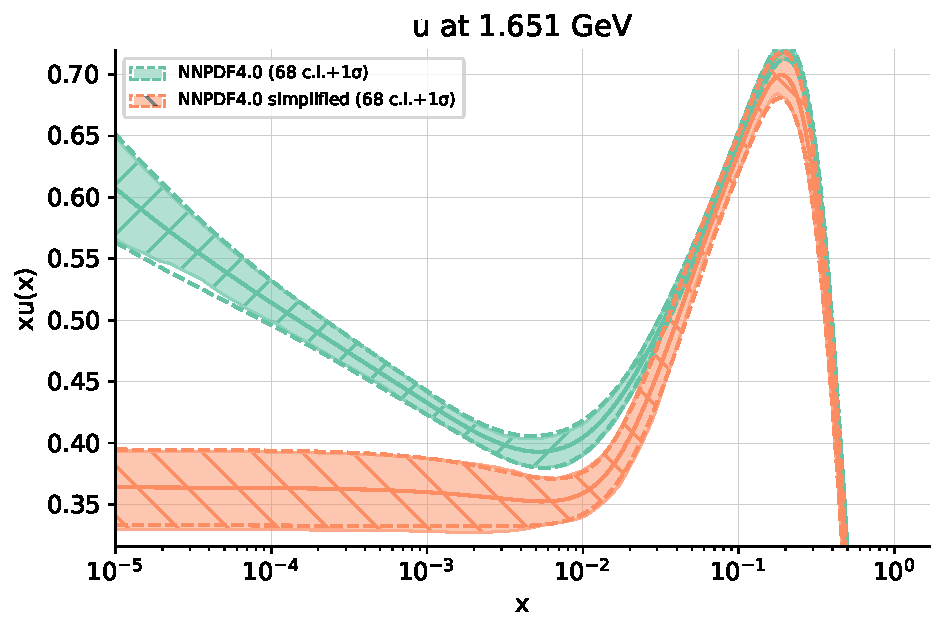
\includegraphics[height=0.55\textheight]{pdf_u_log_saturated.pdf}
    % \\ \nn {\bf What has happened here?}
  \end{center}
\end{frame}


%%%%%%%%%%%%%%%%%%%%%%%%%%%%%%%%%%%%%%%%%%%%%%%%%%%%%%%%%%%%%%%%%%%%%%%%%%%%%%%%%%%%%%%%%%%%%%%%%%%%
\section{Input scaling}


\begin{frame}[t]{Input scaling: The problem}
  Starting from the FK-tables xgrid distribution:\\
  \begin{center}
    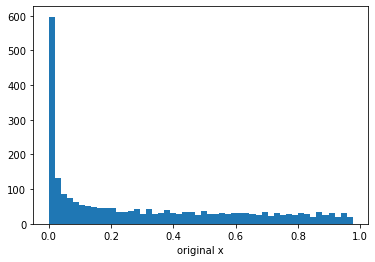
\includegraphics[height=0.4\textheight]{figures/default_xgrid.png}
  \end{center}
  The optimizer is not sensitive for input across multiple orders of magnitude, and without any scaling will only be able to fit features on a linear scale. \\ \nn
  The $(x,\log x)$ input scaling makes the optimizer sensitive to input on a logarithmic scale as well \\ \nn
  We can do better!
\end{frame}


\begin{frame}[t]{Input scaling: The idea}
  Let us take a page from the ML community's playbook.\\
  Equalize the histogram using the empirical cumulative distribution function (CDF):
  \begin{center}
    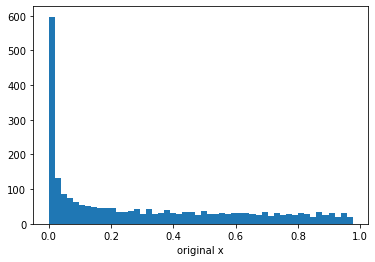
\includegraphics[height=0.4\textheight]{figures/default_xgrid.png} \hspace*{1cm}
    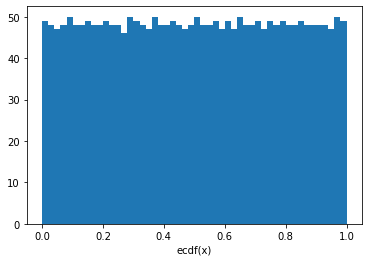
\includegraphics[height=0.4\textheight]{figures/ecdf_xgrid.png}
  \end{center}
  Now data is no longer distributed across many orders of magnitude \\ \nn
  Add an interpolation function and we're done!
\end{frame}


\begin{frame}[t]{Result}
  There appear to be no saturation in the data region:\\
  \begin{center}
    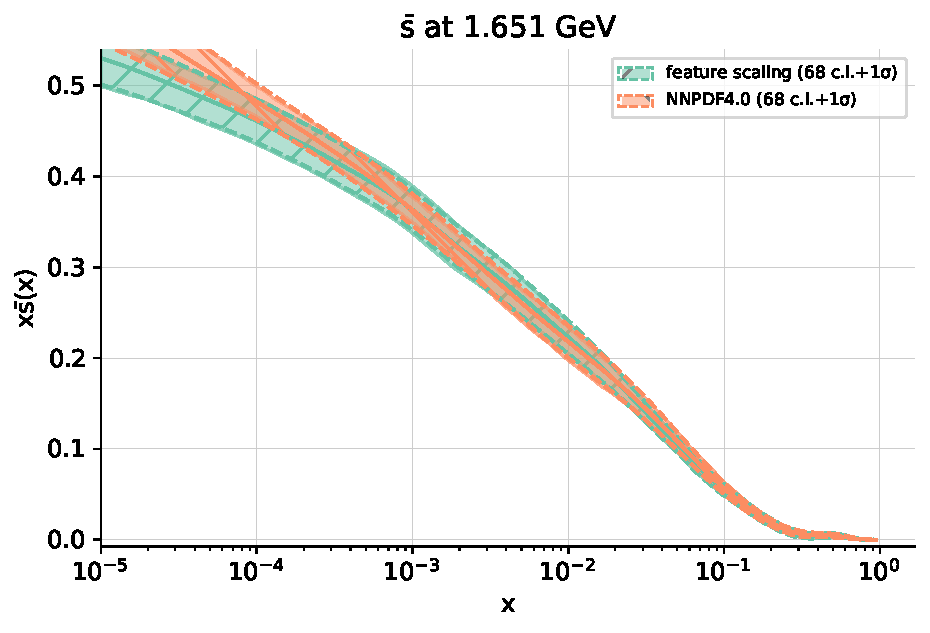
\includegraphics[height=0.5\textheight]{figures/pdf_sbar_log_feature_vs_nnpdf40.pdf}
    \includegraphics[height=0.5\textheight]{pdf_u_log_feature_vs_nnpdf40.pdf}
  \end{center}
  The results shown in this talk remove both preprocessing and $(x,\log x)$, but they should be thought of as independent ideas.
\end{frame}


%%%%%%%%%%%%%%%%%%%%%%%%%%%%%%%%%%%%%%%%%%%%%%%%%%%%%%%%%%%%%%%%%%%%%%%%%%%%%%%%%%%%%%%%%%%%%%%%%%%%
\section{Removing preprocessing}


\begin{frame}[t]{Obstacles to removing preprocessing}
  Getting rid of preprocessing simplifies the model architecture and results in an increased stability between replicas. \\ \nn
  A specific example where this can be beneficial is hyperoptimization (see Juan CM's talk) \\ \nn
  $f(x=1)=0$ is enforced by subtracting the network at $x=1$:\\
  $xf(x)=A_k\left(\mathrm{NN}_k(x) - \mathrm{NN}_k(x=1) \right)$ \\ \nn

  The suggestion of removing preprocessing raises two obvious questions:
  \begin{enumerate}
    \item Can it be done without ruining convergence?
    \item Can the extrapolation region still be trusted?
  \end{enumerate}
  \nn
  \begin{center}
    Let's {\color{blue} \underline{\href{https://vp.nnpdf.science/TVyAUeiNTk26IMYAfRNqLw==}{compare}}} `feature scaling' to NNPDF4.0
  \end{center}
\end{frame}


\begin{frame}[t]{Convergence}
  Statistics are unchanged:\\
  \begin{center}
    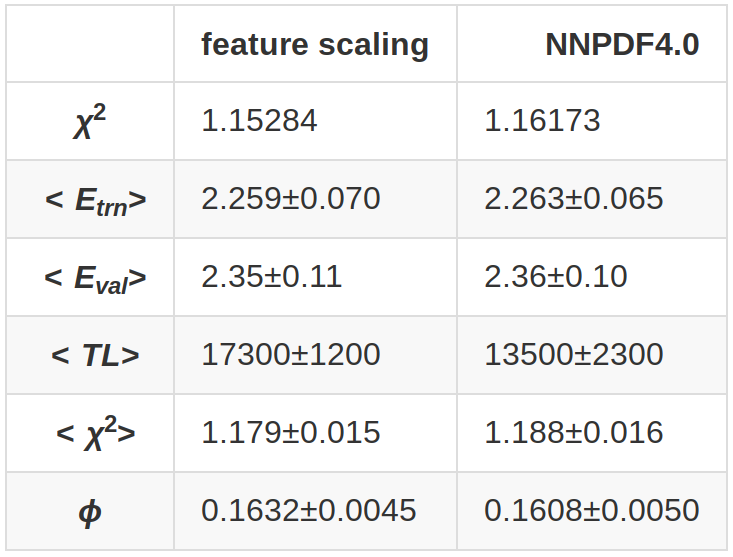
\includegraphics[height=0.5\textheight]{figures/summary_feature_vs_nnpdf40.png}
  \end{center}
\end{frame}


\begin{frame}[t]{Convergence}
  Remember that the PDFs are similar:\\
  \begin{center}
    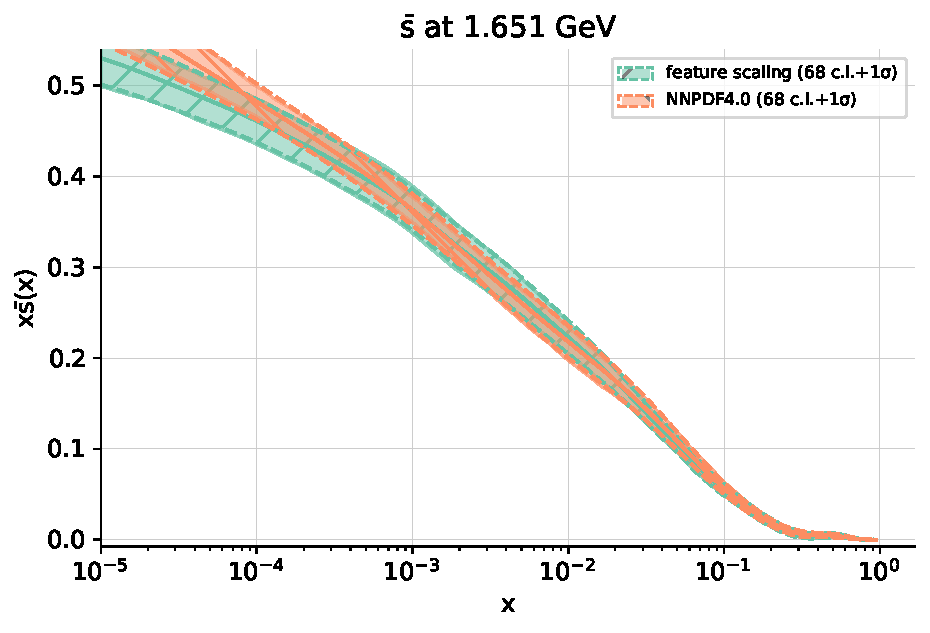
\includegraphics[height=0.5\textheight]{figures/pdf_sbar_log_feature_vs_nnpdf40.pdf}
    \includegraphics[height=0.5\textheight]{figures/pdf_u_log_feature_vs_nnpdf40.pdf}
  \end{center}
\end{frame}


\begin{frame}[t]{The extrapolation region}
  Uncertainty in the extrapolation region is the same:\\
  \begin{center}
    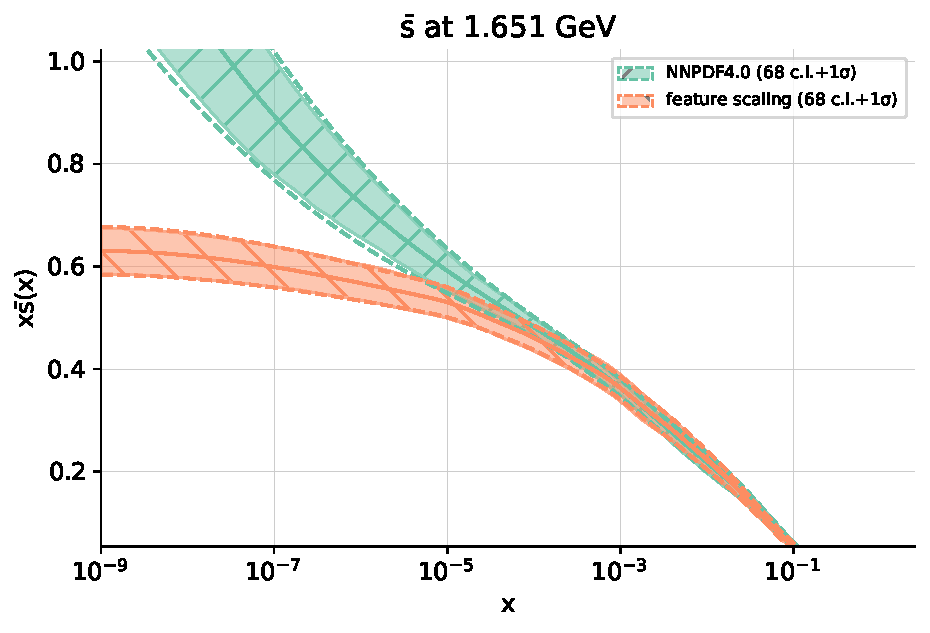
\includegraphics[height=0.5\textheight]{figures/pdf_extra_sbar_feature_vs_nnpdf40.pdf}
    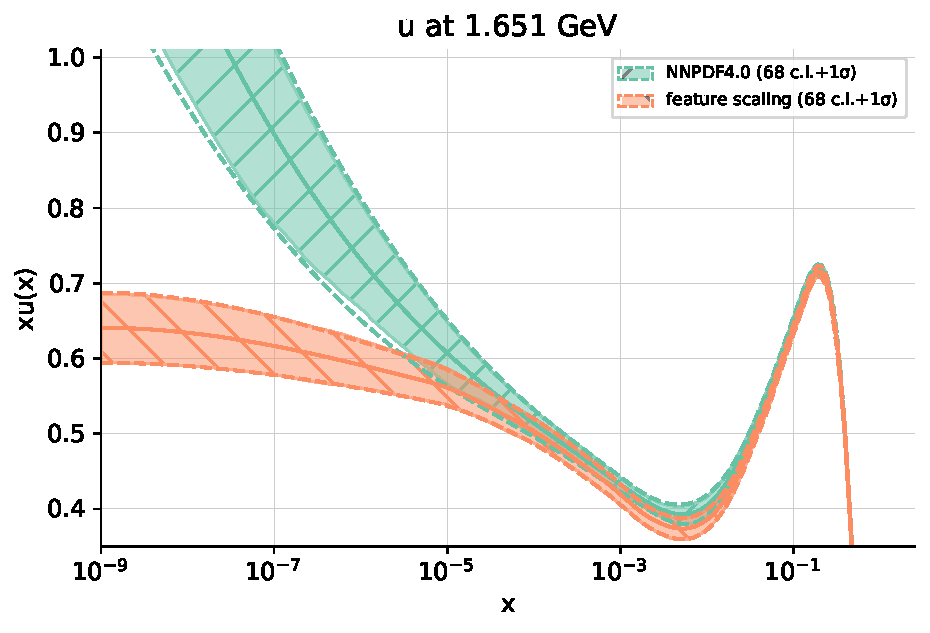
\includegraphics[height=0.5\textheight]{figures/pdf_extra_u_feature_vs_nnpdf40.pdf}
  \end{center}
  Note the plotted range of $x$, LHAPDF grids are provided for $x\geq 10^{-9}$
\end{frame}

\begin{frame}[t]{Future test}
  Let's compare the future tests of {\color{blue} \underline{\href{https://vp.nnpdf.science/ArCroD6xRxmTAGHSBJoD3Q==/}{NNPDF4.0}}} and {\color{blue} \underline{\href{https://vp.nnpdf.science/TVyAUeiNTk26IMYAfRNqLw==}{feature scaling}}} 
  \begin{center}
    \begin{figure}
      \minipage{0.49\textwidth}
        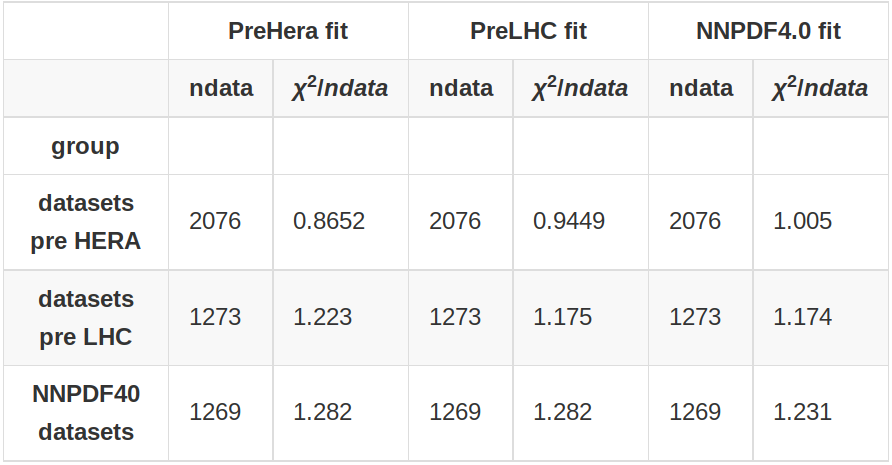
\includegraphics[width=1\textwidth]{figures/futuretest_nnpdf40.png}
        \captionsetup{labelformat=empty}
        \caption{NNPDF4.0}
      \endminipage\hfill
      \minipage{0.49\textwidth}
        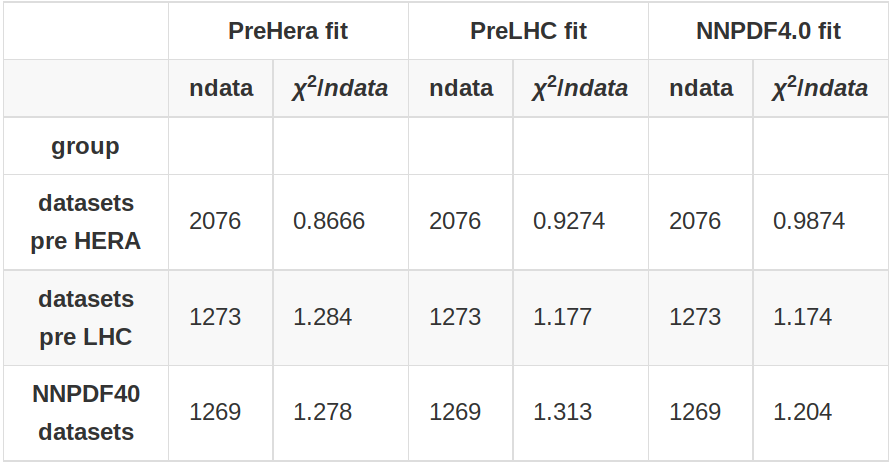
\includegraphics[width=1\textwidth]{figures/futuretest_feature.png}
        \captionsetup{labelformat=empty}
        \caption{feature scaling}
      \endminipage
    \end{figure}
    \vspace*{1em}
    \only<2> {The future test is successful}
  \end{center}
\end{frame}


\begin{frame}[t]{Towards phenomenology: luminosities}
  Good agreement at the level of luminosities:
  \begin{center}
    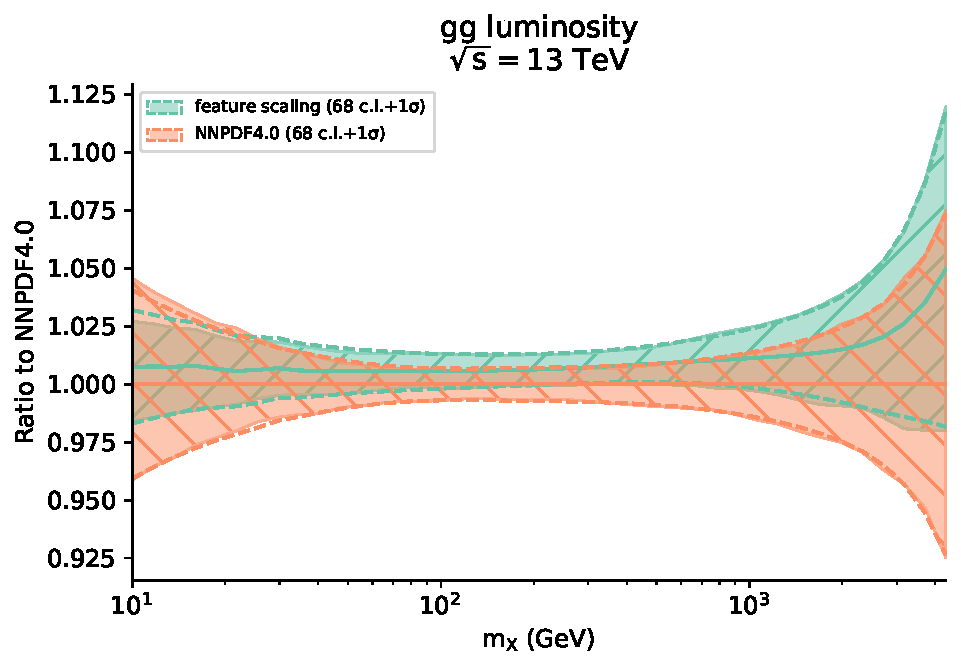
\includegraphics[height=0.5\textheight]{figures/1dlumi_gg_feature_vs_nnpdf40.pdf}
    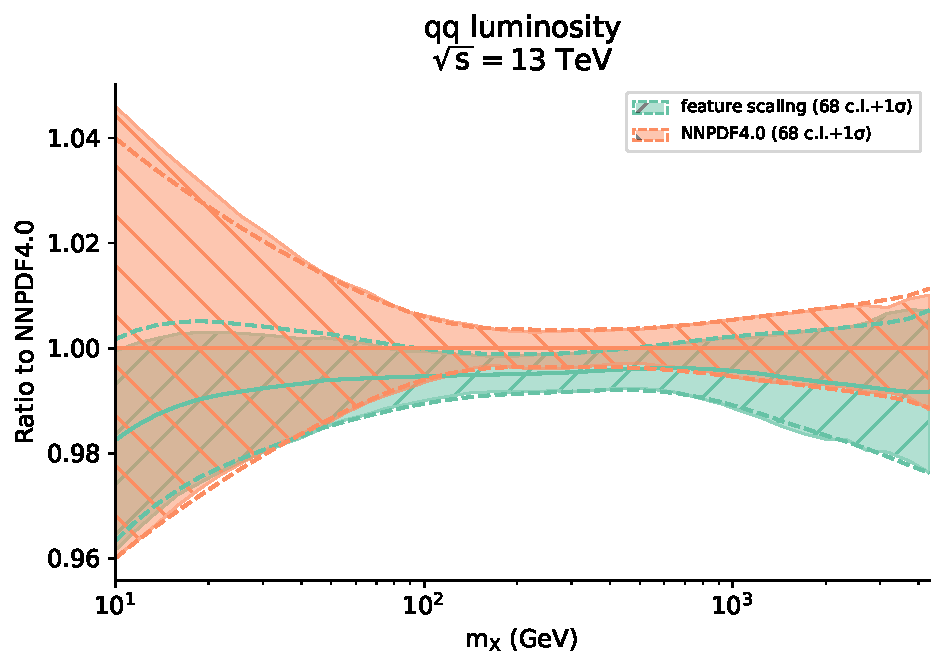
\includegraphics[height=0.5\textheight]{figures/1dlumi_qq_feature_vs_nnpdf40.pdf}
  \end{center}
\end{frame}


\begin{frame}[t]{Phenomenology}{Thanks Christopher for these {\color{blue} \underline{\href{https://vp.nnpdf.science/de96i8VBQ9Gc-zxl75AMfw==/pheno_featurescaling.pdf}{plots}}}}
  Most importantly - good agreement at the level of observables:
  \begin{center}
    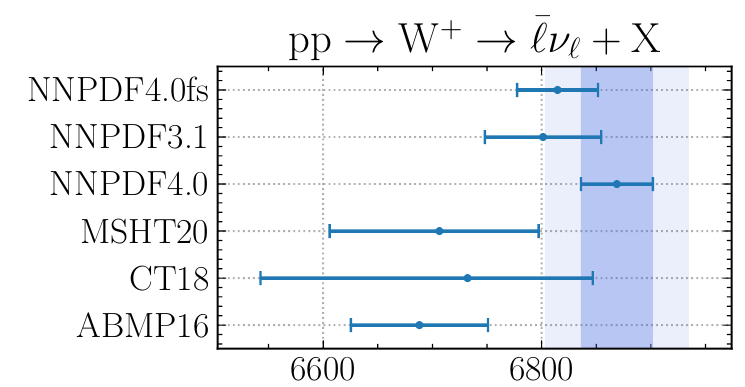
\includegraphics[width=0.4\textwidth]{figures/pheno_w.png} \hfill
    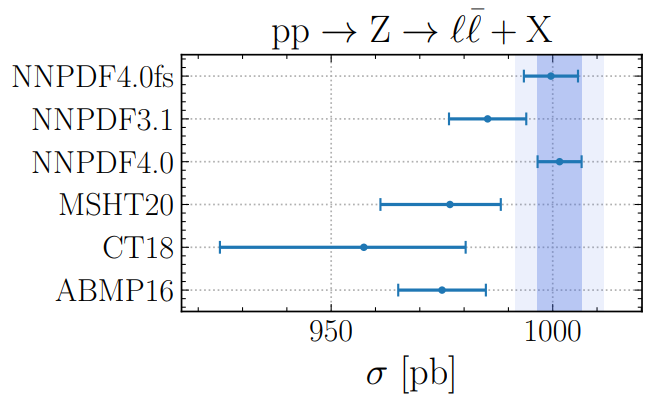
\includegraphics[width=0.4\textwidth]{figures/pheno_z.png}
  \end{center}
  Removing the constraints on the model results in larger uncertainties, while other measures do not deteriorate
\end{frame}



%%%%%%%%%%%%%%%%%%%%%%%%%%%%%%%%%%%%%%%%%%%%%%%%%%%%%%%%%%%%%%%%%%%%%%%%%%%%%%%%%%%%%%%%%%%%%%%%%%%%
\section{Cartomancy: Predicting the extrapolation region}


\begin{frame}[t]{Modelling experimental data}
  Based on an idea proposed during the NNPDF meeting in Amsterdam 2020: see 
  {\color{blue} \underline{\href{https://www.wiki.ed.ac.uk/download/attachments/432523942/carrazza.pdf?version=1&modificationDate=1581344104000&api=v2}{slides}}} \\ \nn
  The proposed small-$x$ strategy is as follows:
  \begin{enumerate}
    \item Select DIS datasets with small-$x$ points
    \item Build a Gaussian Process (GP) model which learns the DIS dataset
    \item Create an xgrid in the small-$x$ extrapolation region
    \item Generate pseudo-data at small-$x$ using the GP model
    \item Compute FK tables for those points
  \end{enumerate} 
\end{frame}



\begin{frame}[t]{Modelling experimental data: Example}
  \begin{center}
    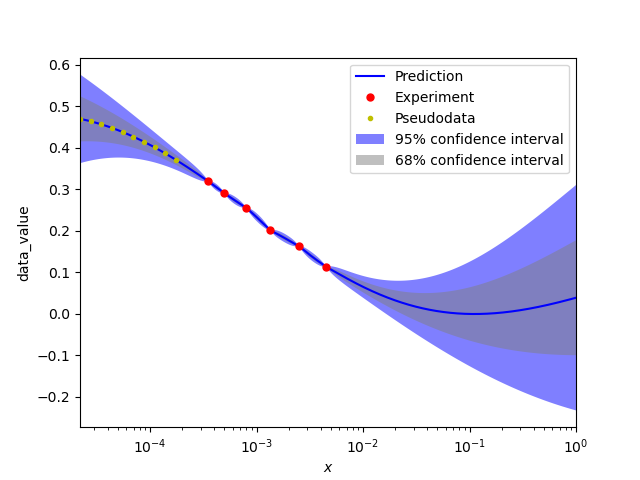
\includegraphics[height=0.6\textheight]{figures/gp_hera.png}
  \end{center}
  Observe that the uncertainty of the psuedo-data is much larger than of the experimental data
\end{frame}


\begin{frame}[t]{Fitting psuedo-data}
  Only with `help' (e.g. artificially increased weight) the psuedo-data can be fitted:
  \begin{center}
    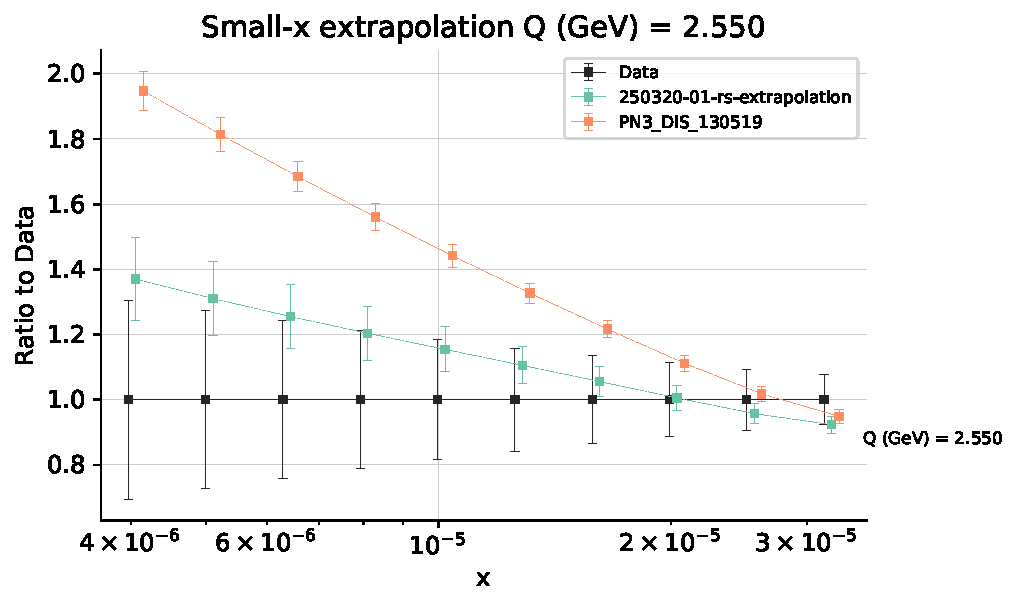
\includegraphics[height=0.5\textheight]{figures/extradata_fitted.pdf}
  \end{center}
  But, even if there is no friction with other datasets, without such help the uncertainties are too large and other datasets dominate the $\chi^2$
\end{frame}


\begin{frame}[t]{Problems}
  \begin{enumerate}
    \item Is there a way to fit data with large uncertainties?
    \item Is the prediction accurate (choice of kernel and parameters)?
    \begin{itemize}
      \item `Future test' the kernels
    \end{itemize}
    % \begin{itemize}
    %   \item Perhaps something along the line of Zahari's ensemble of fits with weighed datasets
    % \end{itemize}
  \end{enumerate}
\end{frame}



%%%%%%%%%%%%%%%%%%%%%%%%%%%%%%%%%%%%%%%%%%%%%%%%%%%%%%%%%%%%%%%%%%%%%%%%%%%%%%%%%%%%%%%%%%%%%%%%%%%%
\bgroup
  \setbeamercolor{background canvas}{bg=RoyBlue}
  \setbeamertemplate{navigation symbols}{}
  \begin{frame}[plain,noframenumbering]{}
    \color{white}
    \huge
    \begin{center}
      \textbf{Thank you!}
    \end{center}
  \end{frame}
\egroup


%%%%%%%%%%%%%%%%%%%%%%%%%%%%%%%%%%%%%%%%%%%%%%%%%%%%%%%%%%%%%%%%%%%%%%%%%%%%%%%%%%%%%%%%%%%%%%%%%%%%
% 
\begin{frame}{Determination of the photon PDF}
  \begin{columns}[T]
    \begin{column}{0.59\textwidth}
      Initially the photon PDF has been determined in different ways:
      \begin{itemize}
        \item physical model: sensitive to underlying model
        \item fitting: data does not provide strong constraints
      \end{itemize}

      \vspace*{0.5em}
      However with the LUXqed approach it can be computed perturbatively \\
      based on the observation that the heavy-lepton production cross-section can be written in two ways:
      \begin{itemize}
        \item in terms of structure functions $F_2$, $F_L$
        \item in terms of PDFs (including the photon)
      \end{itemize}

      \vspace*{0.5em}
      luxQED result {\color{gray}\small[Manohar, Nason, Salam, Zanderighi: 1607.04266, 1708.01256]}:
      \vspace*{-0.8em}
      \begin{equation*}
        \begin{split}
          & x \gamma(x, \mu^2)
          =
          \frac{2}{\alpha (\mu^2)} \int\limits_x^1 \frac{dz}{z}
          \Biggl\{ \int_{m_p^2x^2 \over 1-z}^{\mu^2 \over 1-z} \frac{dQ^2}{Q^2}
          \alpha^2(Q^2) \Biggl[ -z^2 F_L(x/z, Q^2) \\
          & + \left( z P_{\gamma q}(z) + \frac{2 x^2 m_p^2}{Q^2} \right)
          F_2(x/z, Q^2)\Biggr] - \alpha^2(\mu^2) z^2 F_2(x/z, \mu^2)\Biggr\}
        \end{split}
      \end{equation*}
    \end{column}

    \begin{column}{0.39\textwidth}
      \vspace*{-2.5em}
      \begin{figure}
        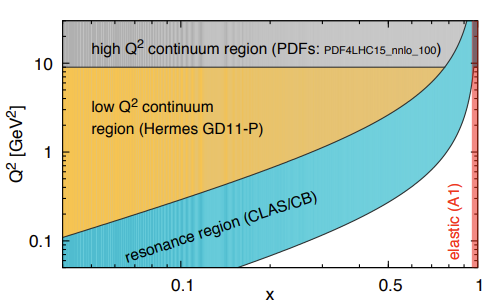
\includegraphics[width=0.89\textwidth]{figures/dataluxqed.png}
        \caption*{Input to construct $F_2$ and $F_L$}
        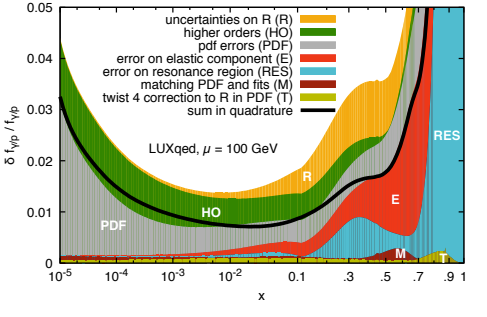
\includegraphics[width=0.89\textwidth]{figures/luxQED_uncs.png}
        \caption*{Sources of uncertainty}
      \end{figure}
    \end{column}
  \end{columns}
\end{frame}


\begin{frame}{LUXqed PDF determinations}
  LUXqed has been used in all of the most recent QED PDFs:
  \begin{itemize}
      \item LUXqed\_plus\_PDF4LHC15 {\color{gray}\small [1607.04266]}
      \item LUXqed17\_plus\_PDF4LHC15 {\color{gray}\small [1708.01256]}
      \item MMHT2015qed {\color{gray}\small [1907.02750]}
      \item NNPDF3.1luxQED {\color{gray}\small [1712.07053]}
      \item CT18lux and CT18qed {\color{gray}\small [2106.10299]}
      \item MSHT20QED {\color{gray}\small [2111.05357]}
      \item MSHT20qed\_an3lo {\color{gray}\small [2312.07665]}
      \item NNPDF4.0QED {\color{gray}\small [2401.08749 ]}
  \end{itemize}
\end{frame}

% \begin{frame}{Results: photon PDF and luminosity}
%   \begin{center}
%     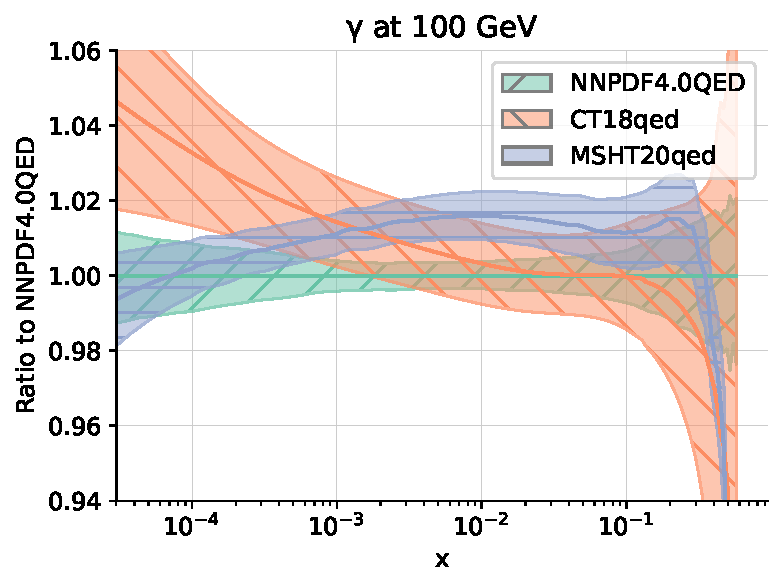
\includegraphics[width=0.3\textwidth]{figures/photon_comparison.pdf}
%     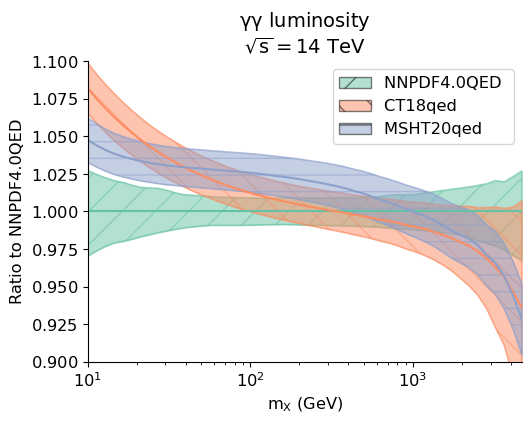
\includegraphics[width=0.3\textwidth]{figures/pp_lumi_comparison.png}
%     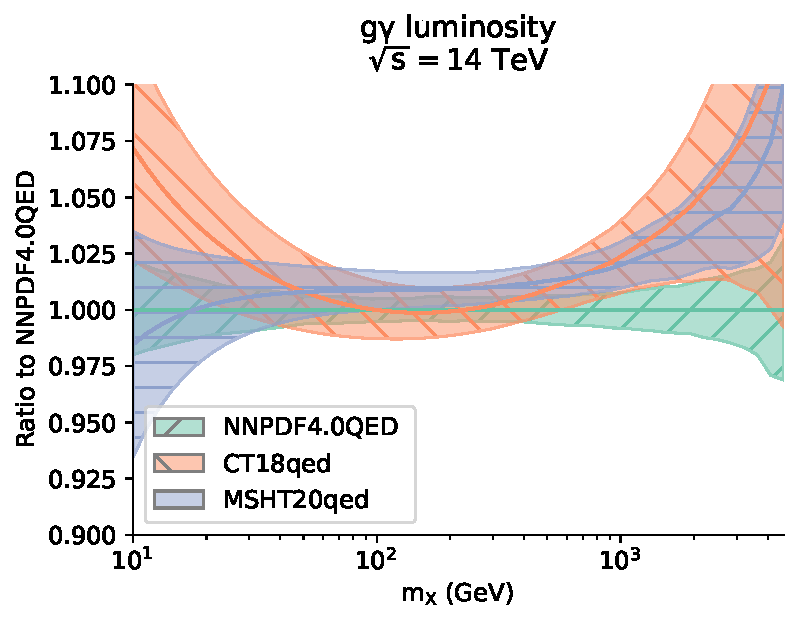
\includegraphics[width=0.3\textwidth]{figures/gp_lumi_comparison.pdf}
%   \end{center}
%   \begin{itemize}
%     \item Because all groups use the luxQED formalism, the photon PDFs agree at percent level
%     \item Luminosity generally in agreement, but differ at very small and very large invariant mass
%   \end{itemize}
% \end{frame}


% ============================================================================


\begin{frame}{Incomplete higher order uncertainties covmat}
  \begin{itemize}
    \item We construct an IHOU matrix following a similar approach by varying the subleading functions
    \item IHOU are independent of MHOU so the uncertainties are added in quadrature
    $$C = C_\mathrm{exp}+C_\mathrm{MHOU}+C_\mathrm{IHOU}$$
  \end{itemize}

  \begin{columns}
    \begin{column}{0.49\textwidth}
      \begin{figure}[!t]
        \centering
        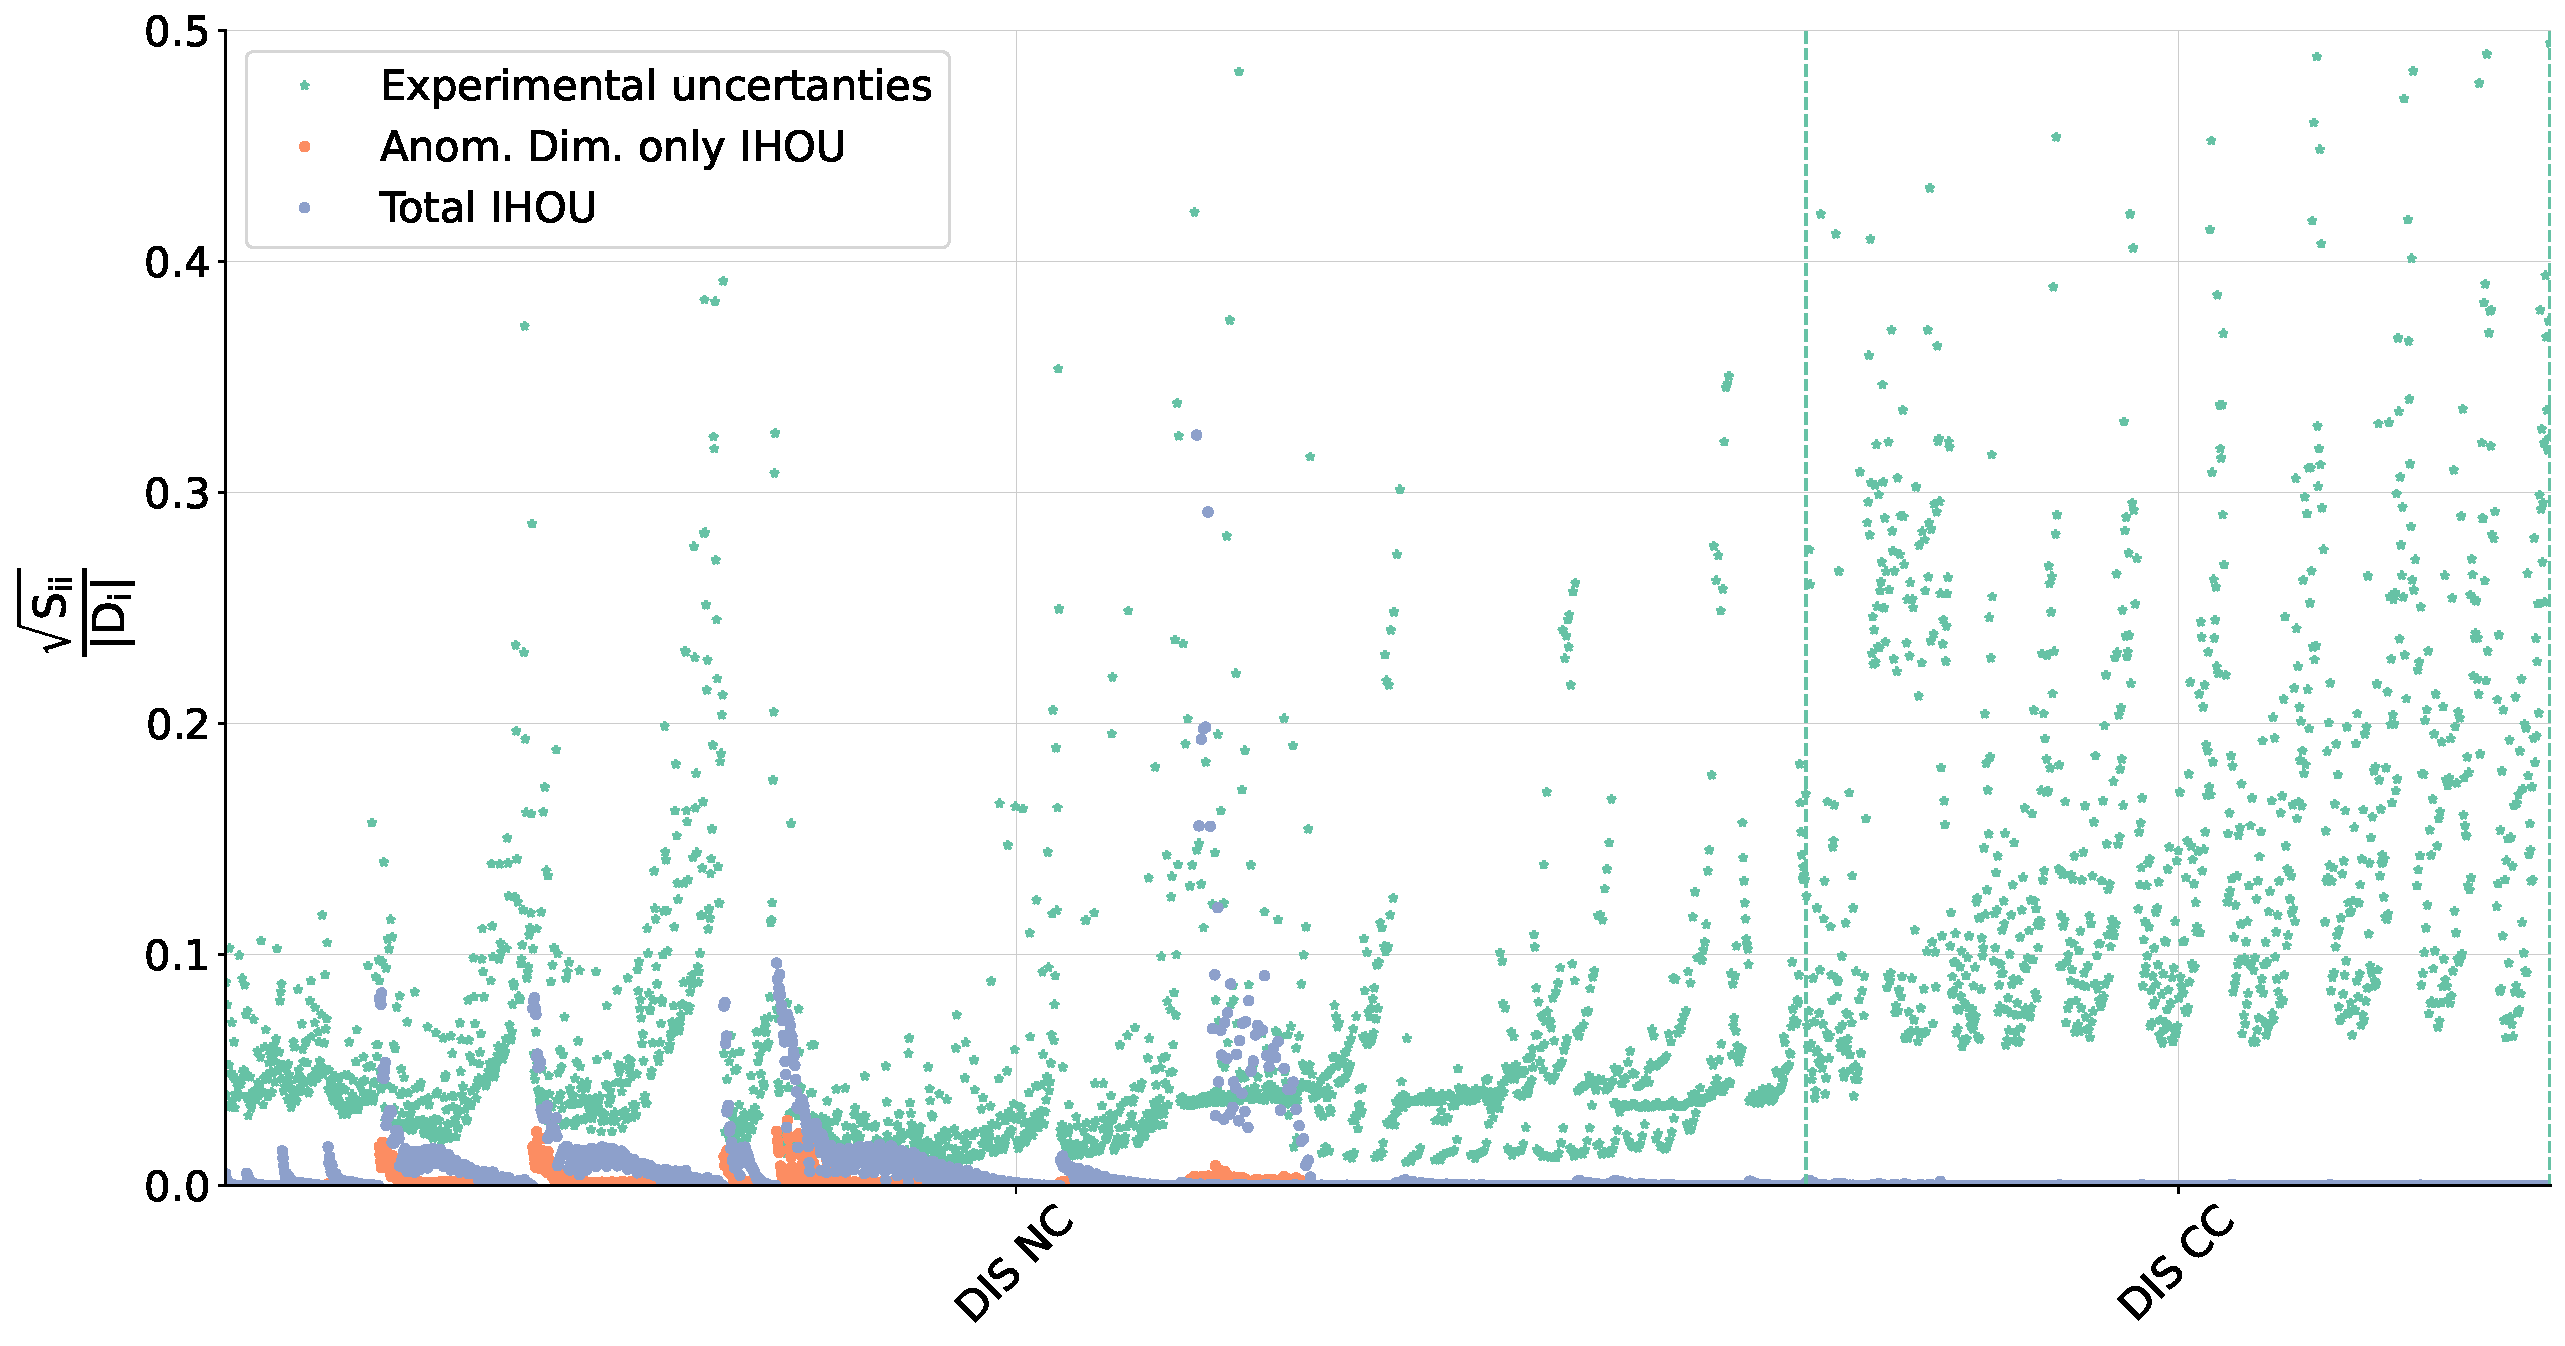
\includegraphics[width=.9\textwidth]{figures/diag_cov_dis_ihou.pdf}
        \caption*{IHOU have a large effect on small-$x$, low-$Q$ DIS data
        }
      \end{figure}
    \end{column}
    \begin{column}{0.49\textwidth}
      \begin{figure}[!t]
        \centering
        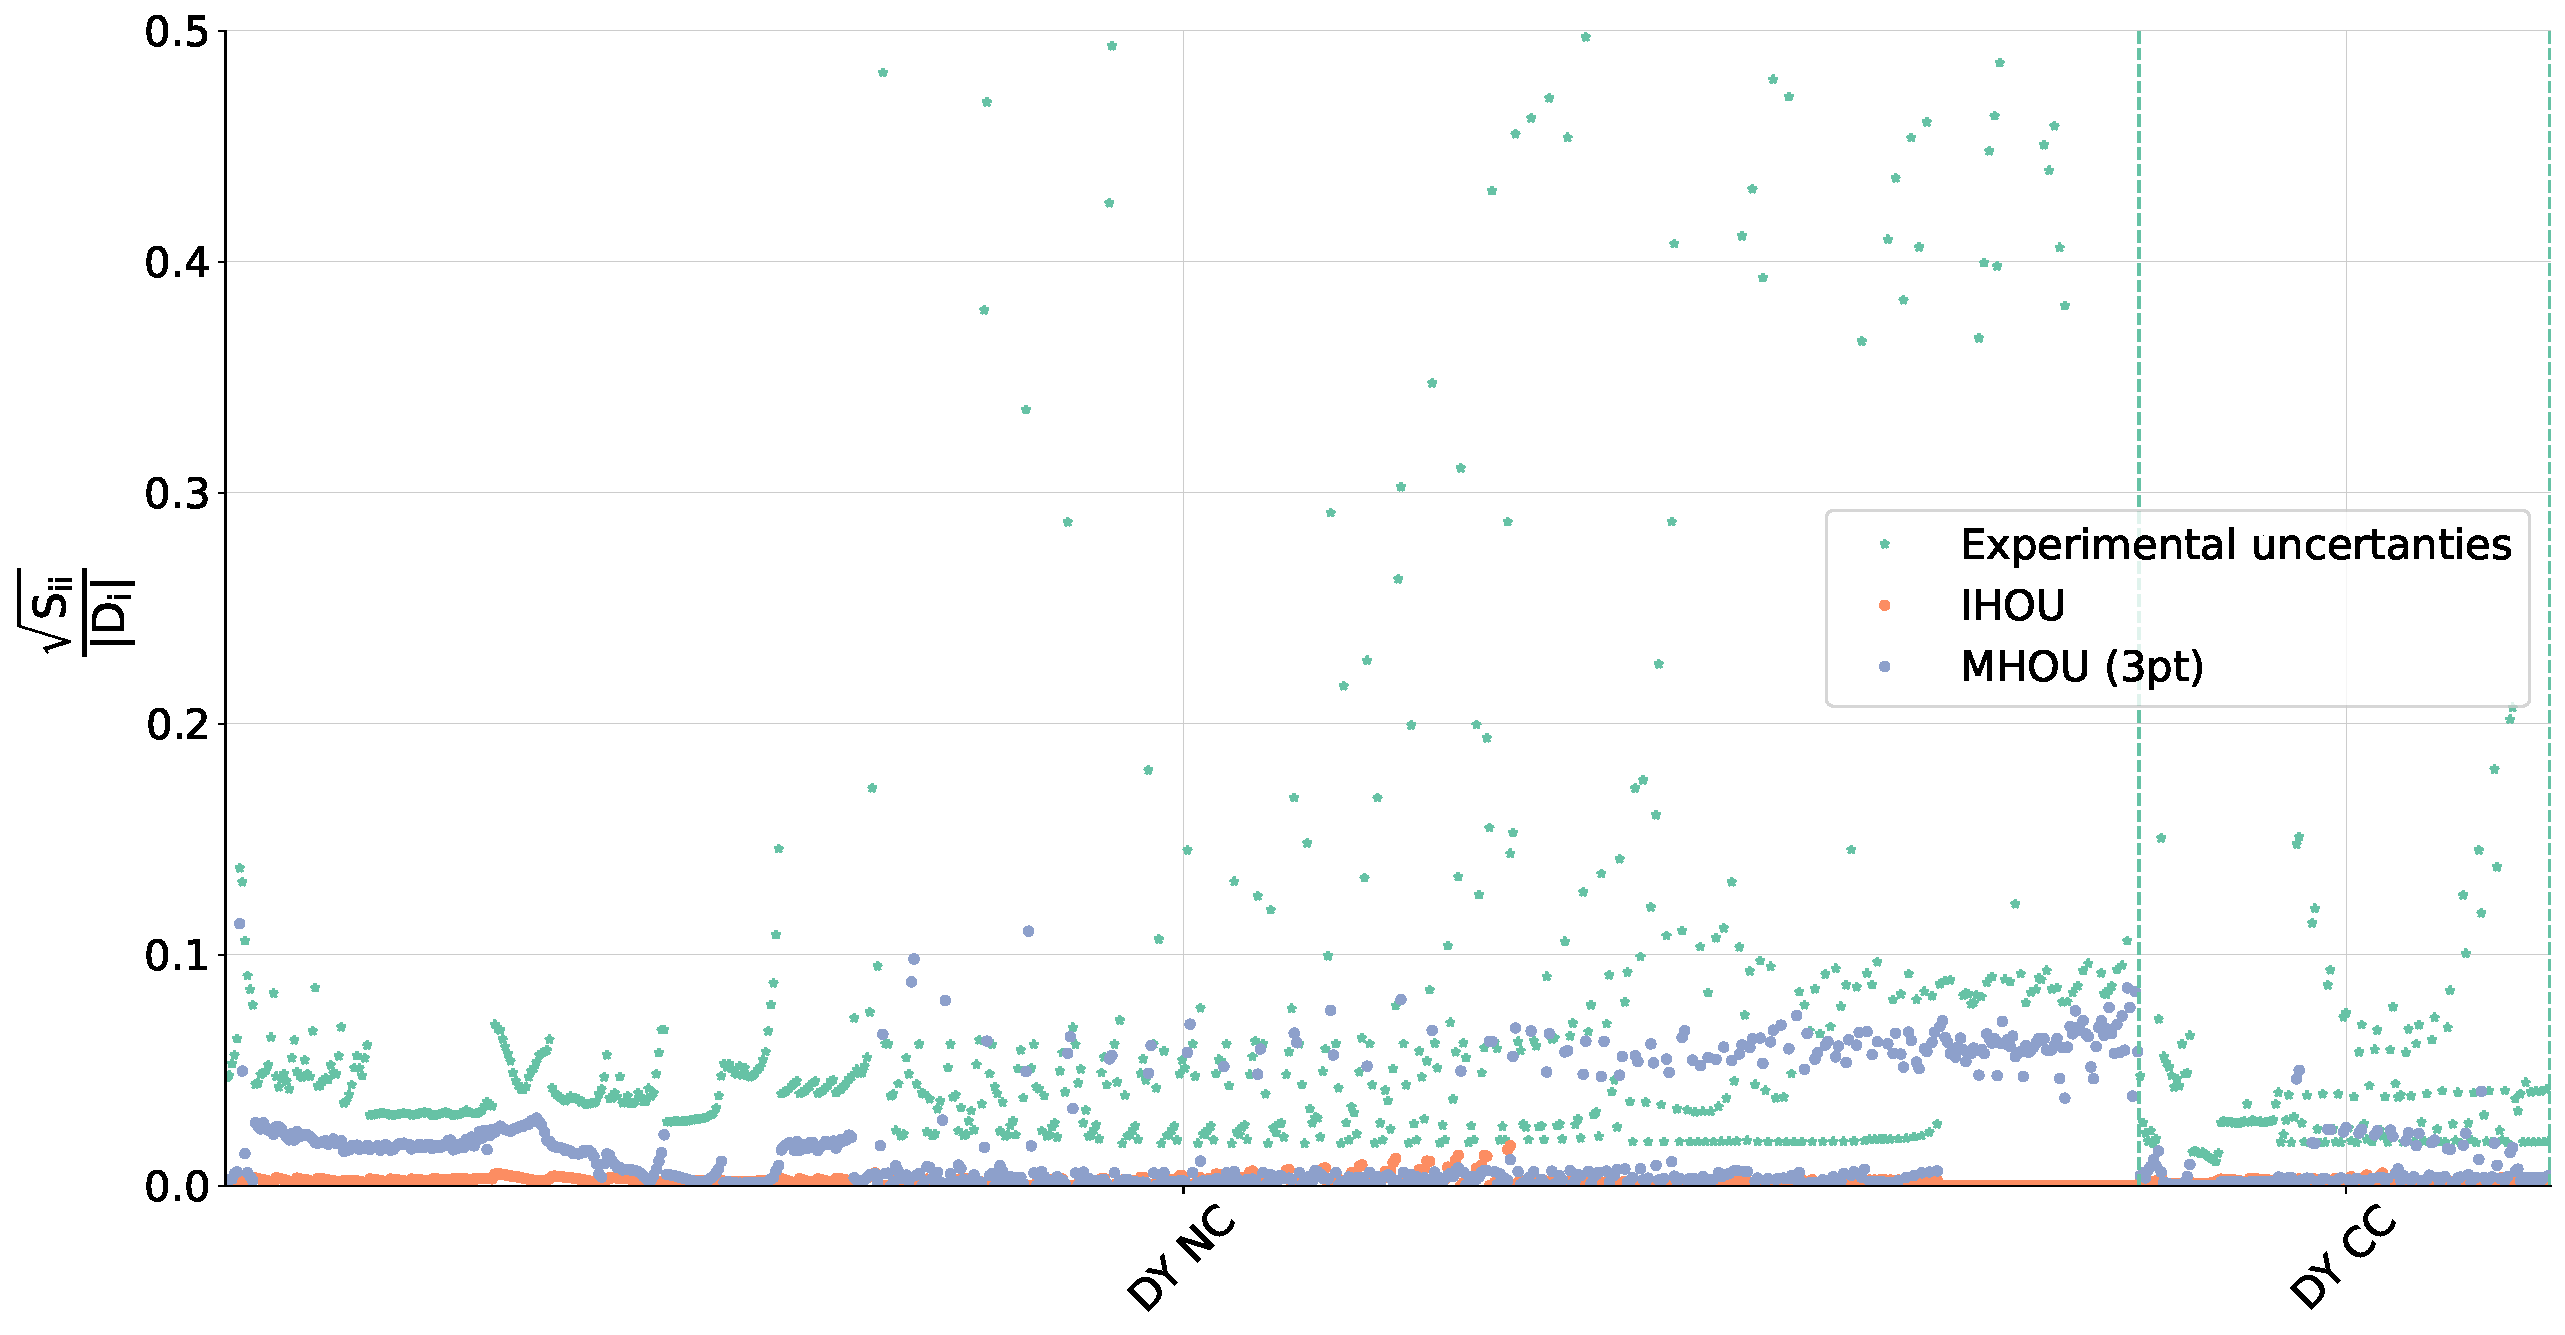
\includegraphics[width=.9\textwidth]{figures/diag_cov_dy_ihou_3pt_mhou.pdf}
        \caption*{NNLO MHOU included where N3LO not available \\
          MHOU can similar magnitude as the experimental uncertainty
        }
      \end{figure}
    \end{column}
  \end{columns}


\end{frame}

% \begin{frame}{Magnitude of theory uncertainties}
% % show that for certain processes th unc is of same size as exp unc.
% \end{frame}

% ============================================================================

\begin{frame}{Impact of MHOUs at N3LO}
  \begin{figure}[!t]
    \centering
    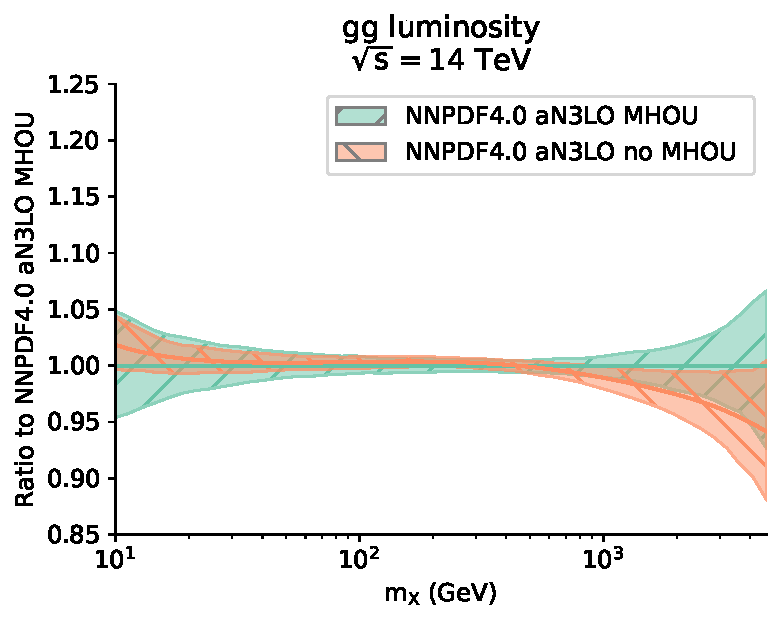
\includegraphics[width=0.45\textwidth]{figures/gg_plot_lumi1d.pdf}
    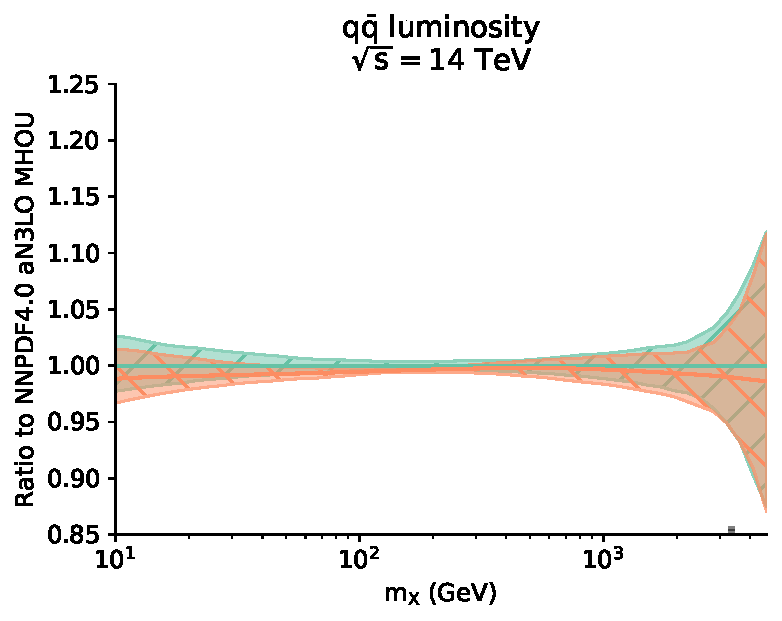
\includegraphics[width=0.45\textwidth]{figures/qqbar_plot_lumi1d.pdf}
  \end{figure}
  \begin{itemize}
    \item Non-negligible impact of MHOUs even at N3LO
    \item[$\Rightarrow$] reason to include exact N3LO calculations for hadronic processes
  \end{itemize}
\end{frame}


% \begin{frame}{Comparison to MSHT20}
%   \begin{figure}[!t]
%     \centering
%     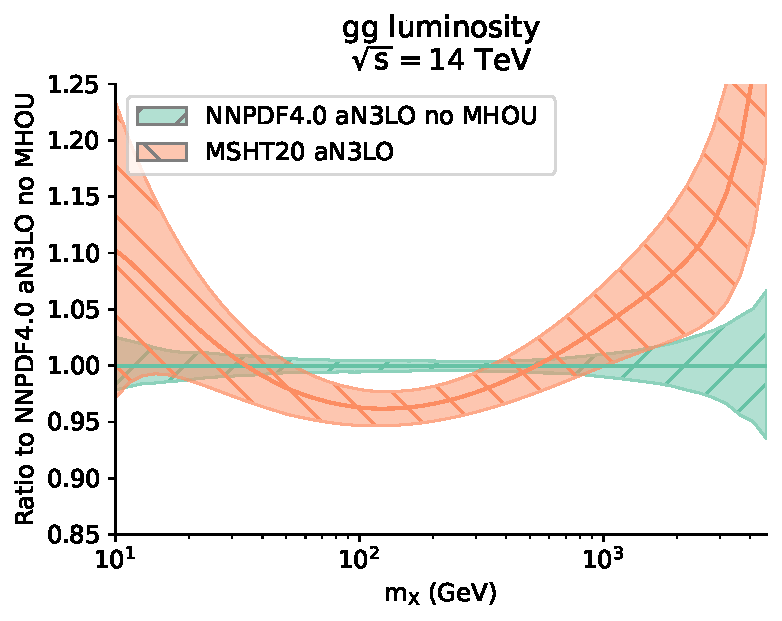
\includegraphics[width=0.45\textwidth]{figures/gg_plot_lumi1d_msht20.pdf}
%     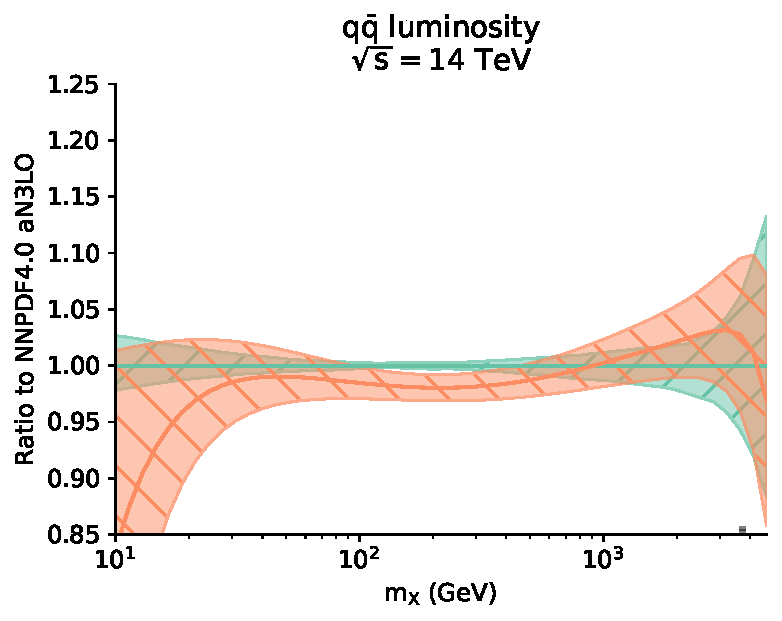
\includegraphics[width=0.45\textwidth]{figures/qqbar_plot_lumi1d_msht20.pdf}
%   \end{figure}
%   \begin{itemize}
%     \item Good agreement with MSHT20 for the quark luminosities
%     \item Also for gluon luminosities, except around the Higgs mass and high-mass
%     \item Similar data but different methodology (including splitting function parametrization)
%   \end{itemize}
% \end{frame}



\end{document}
